%Version 2.1 April 2023
% See section 11 of the User Manual for version history
%
%%%%%%%%%%%%%%%%%%%%%%%%%%%%%%%%%%%%%%%%%%%%%%%%%%%%%%%%%%%%%%%%%%%%%%
%%                                                                 %%
%% Please do not use \input{...} to include other tex files.       %%
%% Submit your LaTeX manuscript as one .tex document.              %%
%%                                                                 %%
%% All additional figures and files should be attached             %%
%% separately and not embedded in the \TeX\ document itself.       %%
%%                                                                 %%
%%%%%%%%%%%%%%%%%%%%%%%%%%%%%%%%%%%%%%%%%%%%%%%%%%%%%%%%%%%%%%%%%%%%%

\documentclass[sn-vancouver,Numbered,pdflatex]{sn-jnl}

%%%% Standard Packages
%%<additional latex packages if required can be included here>

\usepackage{graphicx}%
\usepackage{multirow}%
\usepackage{amsmath,amssymb,amsfonts}%
\usepackage{amsthm}%
\usepackage{mathrsfs}%
\usepackage[title]{appendix}%
\usepackage{xcolor}%
\usepackage{textcomp}%
\usepackage{manyfoot}%
\usepackage{booktabs}%
\usepackage{algorithm}%
\usepackage{algorithmicx}%
\usepackage{algpseudocode}%
\usepackage{listings}%
%%%%

%%%%%=============================================================================%%%%
%%%%  Remarks: This template is provided to aid authors with the preparation
%%%%  of original research articles intended for submission to journals published
%%%%  by Springer Nature. The guidance has been prepared in partnership with
%%%%  production teams to conform to Springer Nature technical requirements.
%%%%  Editorial and presentation requirements differ among journal portfolios and
%%%%  research disciplines. You may find sections in this template are irrelevant
%%%%  to your work and are empowered to omit any such section if allowed by the
%%%%  journal you intend to submit to. The submission guidelines and policies
%%%%  of the journal take precedence. A detailed User Manual is available in the
%%%%  template package for technical guidance.
%%%%%=============================================================================%%%%

%% Per the spinger doc, new theorem styles can be included using built in style, 
%% but it seems the don't work so commented below
%\theoremstyle{thmstyleone}%
\newtheorem{theorem}{Theorem}%  meant for continuous numbers
%%\newtheorem{theorem}{Theorem}[section]% meant for sectionwise numbers
%% optional argument [theorem] produces theorem numbering sequence instead of independent numbers for Proposition
\newtheorem{proposition}[theorem]{Proposition}%
%%\newtheorem{proposition}{Proposition}% to get separate numbers for theorem and proposition etc.

%% \theoremstyle{thmstyletwo}%
\theoremstyle{remark}
\newtheorem{example}{Example}%
\newtheorem{remark}{Remark}%

%% \theoremstyle{thmstylethree}%
\theoremstyle{definition}
\newtheorem{definition}{Definition}%

\usepackage{float}
\let\origfigure\figure
\let\endorigfigure\endfigure
\renewenvironment{figure}[1][2] {
    \expandafter\origfigure\expandafter[H]
} {
    \endorigfigure
}
\usepackage{lscape}
\usepackage{pdflscape}
\newcommand{\blandscape}{\begin{landscape}}
\newcommand{\elandscape}{\end{landscape}}
\usepackage[none]{hyphenat}
\usepackage[export]{adjustbox}
\usepackage{multirow}
\usepackage{longtable}
\usepackage{array}
\usepackage{wrapfig}
\usepackage{colortbl}
\usepackage{booktabs} 
\usepackage{colortbl}
\usepackage{pdflscape}
\usepackage{tabu}
\usepackage{threeparttable}
\usepackage[normalem]{ulem}
\usepackage{threeparttablex}
\usepackage{makecell}



\raggedbottom




% tightlist command for lists without linebreak
\providecommand{\tightlist}{%
  \setlength{\itemsep}{0pt}\setlength{\parskip}{0pt}}

% From pandoc table feature
\usepackage{longtable,booktabs,array}
\usepackage{calc} % for calculating minipage widths
% Correct order of tables after \paragraph or \subparagraph
\usepackage{etoolbox}
\makeatletter
\patchcmd\longtable{\par}{\if@noskipsec\mbox{}\fi\par}{}{}
\makeatother
% Allow footnotes in longtable head/foot
\IfFileExists{footnotehyper.sty}{\usepackage{footnotehyper}}{\usepackage{footnote}}
\makesavenoteenv{longtable}




\begin{document}


\title[Transparent, reusable and updatable computational models]{A prototype software framework for transparent, reusable and updatable computational health economic models}

%%=============================================================%%
%% Prefix	-> \pfx{Dr}
%% GivenName	-> \fnm{Joergen W.}
%% Particle	-> \spfx{van der} -> surname prefix
%% FamilyName	-> \sur{Ploeg}
%% Suffix	-> \sfx{IV}
%% NatureName	-> \tanm{Poet Laureate} -> Title after name
%% Degrees	-> \dgr{MSc, PhD}
%% \author*[1,2]{\pfx{Dr} \fnm{Joergen W.} \spfx{van der} \sur{Ploeg} \sfx{IV} \tanm{Poet Laureate}
%%                 \dgr{MSc, PhD}}\email{iauthor@gmail.com}
%%=============================================================%%

\author*[1,2]{\pfx{Dr.} \fnm{Leading} \spfx{van} \sur{Author} \sfx{III} \tanm{Poet Laureate} \dgr{MSc, PhD}}\email{\href{mailto:abc@def}{\nolinkurl{abc@def}}}

\author[2]{\fnm{Second} \sur{Author} }



  \affil*[1]{\orgdiv{Department}, \orgname{Organization}, \orgaddress{\city{City}, \country{Country}, \postcode{100190}, \state{State}, \street{Street}}}
  \affil*[2]{\orgname{Other Organisation}}

\abstract{\textbf{Summary: } Most health economic analyses are undertaken with the aid of computers. However, the ethical dimensions of implementing health economic models as software (or computational health economic models (CHEMs)) are poorly understood. We propose that developers and funders of CHEMs share ethical responsibilities to (i) establish socially acceptable user requirements and design specifications; (ii) ensure fitness for purpose; and (iii) support socially beneficial use. We further propose that a transparent (T), reusable (R) and updatable (U) CHEM is suggestive of a project team that has largely fulfilled these responsibilities. We propose six criteria for assessing CHEMs: (T1) software files are open access; (T2) project team contributions and judgments are easily identified; (R1) programming practices promote generalisability and transferability; (R2) licenses restrict only unethical reuse; (U1) maintenance infrastructure is in place; and (U2) new releases are systematically retested and appropriately deprecated. To facilitate CHEMs that meet TRU criteria, we have developed a prototype software framework in the open-source programming language R. The framework comprises six code libraries for authoring CHEMs, supplying CHEMs with data and undertaking analyses with CHEMs. The prototype software framework integrates with services for software development and research data archiving. We determine that an initial set of youth mental health CHEMs we developed with the prototype software framework wholly meet criteria T1-2, R1-2 and U1 and partially meet criterion U2. Our assessment criteria and prototype software framework can help inform and improve ethical implementation of CHEMs. Resource barriers to ethical CHEM practice should be addressed by research funders. \newline \newline \textbf{Code: } Visit \url{https://www.ready4-dev.com} for more information about how to find, install and apply the prototype software framework and CHEMs developed with it. \newline \newline}

\keywords{key, dictionary, word}


\pacs[JEL Classification]{D8, H51}
\pacs[MSC Classification]{35A01, 65L10}

\maketitle

\hypertarget{introduction}{%
\section{Introduction}\label{introduction}}

Health economics is a discipline concerned with problems that arise due to scarce resources, such as how to value health and healthcare, allocate healthcare budgets and configure health services \citep{wagstaff2012four}. In seeking to solve these problems, health economists typically use models which are simplified and selective representations of systems that are believed to influence human health. A health economic model should be capable of being described using words and figures (a conceptual model), equations (a mathematical model) and software (a computational model). Health economic scientific manuscripts typically describe a model using its conceptual and mathematical representations but report results that have been generated by its computational representation (i.e., the format that allows computers to perform calculations). The conceptual, mathematical and computational representations of a model are assumed to be isomorphic. However, the ease of independently assessing the validity of this assumption depends in part on how a health economic model has been implemented computationally.

The set of software files implementing a health economic model's structure, data and algorithms can be called a computational health economic model (CHEM). CHEMs can be developed using commercial modelling software or open-source programming languages such as Python \citep{python2009} or R \citep{RCORE2022}. An advantage of commercial modelling software is that users often require limited or no programming skills to develop and apply CHEMs. However, open-source software programming languages may facilitate the development of CHEMs that are more transparent, reusable and updatable \citep{incerti2019r, Pouwels2022}. The decision about what type of software development platform to use must balance ethical considerations and resource constraints (see Table \ref{tab:proscons}).

Open-source CHEMs remain rare \citep{Feenstra2022, Emerson2019}. The software used to develop CHEMs was identified as a barrier to open-source model implementations by participants in a 2020 survey of health economists \citep{Pouwels2022}. Other reported barriers relate to difficulties in generalising models, updating models and transferring model data, concerns about the level of public access and lack of interest from decision-makers, and legal, confidentiality and security considerations \citep{Pouwels2022}.

Better software frameworks could potentially help address some of the barriers to open-source CHEM development. A software framework is a shared common technology used by developers to collaboratively author software and which is not typically visible to software end-users \citep{myllarniemi2018development}. A software framework provides a foundation for developing multiple software applications with shared resources (e.g., code and data files), that can be modified to suit specific needs. Advantages of using software frameworks include facilitating code reuse and extension, promoting good programming practice and the capability to provide enhanced functionality and performance without additional effort by developers \citep{edwin2014software}. Software frameworks have widely been developed and implemented in data science, for example, PyTorch \citep{PyTorch2019} for machine learning using Python.

A high-level software framework for implementing open-source CHEMs in R has previously been developed with the primary aim of improving model transparency \citep{alarid2019need}. However, to gain widespread adoption, a software framework for CHEMs may need to provide tools to help model developers meet a broader range of ethical practice requirements. There are multiple challenges to overcome. Firstly, the ethical responsibilities of public health computational modellers remain poorly understood \citep{10.3389/fpubh.2017.00068} and the computational modelling landscape is changing fast \citep{calder2018computational}. Secondly, software frameworks can be challenging and time consuming to create and may become excessively complex over time \citep{edwin2014software}. Thirdly, software frameworks can be difficult to learn, often requiring model developers to undergo specialist training \citep{myllarniemi2018development}.

In this paper, we:

\begin{enumerate}
\def\labelenumi{(\roman{enumi})}
\item
  propose a set of ethical responsibilities for CHEM project teams and criteria for assessing ethical CHEM implementations;
\item
  describe a prototype software framework we have developed to support the ethical implementation of CHEMs; and
\item
  assess an initial set of youth mental health CHEMs developed with our software framework against our proposed ethical CHEM implementation criteria.
\end{enumerate}

\hypertarget{ethical-issues}{%
\section{Ethical issues}\label{ethical-issues}}

We considered literature on modelling practice and reflected on our prior experience with developing and using CHEMs to identify: (i) some core ethical responsibilities of CHEM project teams; (ii) attributes of CHEMs that can suggest fulfillment of these responsibilities; and (iii) criteria against which these attributes can be assessed.

\hypertarget{ethical-responsibilities-of-chem-project-teams}{%
\subsection{Ethical responsibilities of CHEM project teams}\label{ethical-responsibilities-of-chem-project-teams}}

Boden and McKendrick \citep{10.3389/fpubh.2017.00068} propose a framework for ethical public health modelling based on the criteria of independence (concerning how modeller subjectivity shapes model design), beneficence / non-maleficence (concerning model quality and utility), transparency (concerning the need for policymakers to reliably evaluate model strengths and weaknesses) and justice (concerning the social obligations of modellers to consider and communicate ethical issues about model use). However, these criteria are not specific to the computational model, but are designed to apply to a modelling project as a whole, including a model's conceptual and mathematical representations. The authors propose 13 questions to evaluate ethical risk across the four criteria, but of these, only ``is the model code open source or available on request'' (for transparency) and ``has the model been verified, i.e., does it do what the modeller wants it to do?'' (for beneficence / non-maleficence) are specific to model's representation as software.

To identify ethical issues that are specific to CHEMs, we first considered the distinct phases in a software development project. Software development lifecycle (SDLC) models take different approaches to the inclusion, naming, definition, sequencing and iteration of project phases \citep{ruparelia2010software}. However, SDLC models typically have components that can principally map to the concepts of \emph{planning} (e.g., identification of system / user requirements and design specifications), \emph{implementation} (e.g., development and testing) and \emph{release} (e.g., deployment, system integration, maintenance and support). For simplicity, we propose one overarching ethical responsibility for CHEM project teams for each phase. These responsibilities are to:

\begin{enumerate}
\def\labelenumi{(\roman{enumi})}
\item
  \textbf{establish socially acceptable user requirements and design specifications} (during CHEM planning);
\item
  \textbf{ensure fitness for purpose} (of CHEM implementation); and
\item
  \textbf{support socially beneficial use} (on CHEM release).
\end{enumerate}

Transparency underpins all three responsibilities (Table \ref{tab:timelygls}). Boden and McKendrick's other ethical criteria can be selectively mapped to each phase's responsibility: justice and independence to the planning responsibility; independence to the implementation responsibility; and beneficence / non-maleficence and justice to the release responsibility. All three ethical responsibilities have implications for both professional practice and project resourcing. As it is unreasonable to place expectations of modellers that they are not resourced to fulfil, these responsibilities should apply jointly to health economic model developers and funders.

Misalignment between the values of computational model developers and those of the population groups affected by decisions based on their models presents significant ethical risks \citep{thompson2022escape, duckett2022journey}. The value judgments of health economic modellers are rarely adequately specified, omissions that may lead to socially unacceptable policy recommendations \citep{duckett2022journey}. These value judgments influence the assumptions, selection of model features and standards for evidence that shape health economic model projects \citep{HARVARD2020112975}. For example, as illustrated in Table \ref{tab:proscons}, project resource constraints may require model developers to make trade-offs when agreeing CHEM \textbf{user requirements and design specifications}. These trade-offs in turn determine how straightforward it is for a CHEM to be subsequently amended to reflect alternative value judgments relating to model conceptualisation and mathematical formalisation (Table \ref{tab:timelygls}).

Modellers have duties both to ensure a computational model is \textbf{fit for purpose} and to provide potential third-party users with the means of assessing its adequacy for their proposed uses \citep{Erdemir2020, Feenstra2022, thompson2019escape, 10.3389/fpubh.2017.00068}. However, it is common for health economic models to have serious methodological flaws \citep{carletto_zanuzzi_sammarco_russo_2020, WONDER2015467}; insufficient validation \citep{Ghabri2019, kolovos2017model, haji2013model}, poor reproducibility \citep{Jalali2021, McManus2019, Bermejo2017}; and undeclared errors \citep{Radeva2020}. Appropriate computational implementation choices can help address many of these shortcomings, for example by automating quality assurance checks and facilitating manual reviews by third parties.

A CHEM will have limited \textbf{social benefit} if it is rarely used, if mis-used or when its acceptability and adequacy rapidly decay. Reuse of CHEMs as components of other models can potentially make model development more efficient \citep{Arnold2010, garcia2021cost}. However, health economic models face challenges related to transferability across jurisdictions \citep{garcia2021cost} that create barriers to reuse. Without ongoing maintenance, a CHEM risks becoming less reliable with time \citep{garcia2021cost} and is at risk of being deployed for purposes for which it is poorly suited \citep{calder2018computational}. Currently, health economic models are rarely implemented computationally in a manner that facilitates routine updates \citep{Sampson2017}, thus limiting the temporal window within which a CHEM can be validly applied.

\hypertarget{chem-attributes-associated-with-ethical-modelling-practice}{%
\subsection{CHEM attributes associated with ethical modelling practice}\label{chem-attributes-associated-with-ethical-modelling-practice}}

The responsibilities of model project teams over a CHEM lifecycle are easier to state than to measure. However, aspects of ethical modelling practice may be inferred from measurable attributes of CHEMs. As described in Table \ref{tab:timelygls}, we believe that the creators of transparent, reusable and updatable (TRU) CHEMs are likely to have fulfilled a number of their ethical obligations. We therefore selected these model attributes to use as the basis for deriving ethical assessment criteria.

Taking steps to make computational models \textbf{transparent} is an important part of ethical public health modelling practice \citep{10.3389/fpubh.2017.00068}. Guidance on transparency in health economic modelling recommend that model code and data should be clearly documented \citep{Eddy2012}. Notably, the same guidelines, published over ten years ago, do not recommend sharing model code and data. However, more recent healthcare modelling guidance does recommend public dissemination of such artefacts \citep{Erdemir2020}. Online repository services such as Zenodo \citep{Zenodo2013} and Dataverse \citep{Dataverse2007} provide persistent storage solutions that generate a Digital Object Identifier (DOI) for each code and data collection. Ensuring that calculations are correct and consistent with model specifications is an essential part of CHEM quality assurance \citep{techver2019}. The extensiveness of such verification checks can be reported using the concept of code coverage \citep{ERICWONG2010188} - the proportion of model code that has been explicitly tested. Tests should ideally combine both unit tests (to verify that small, isolated sections of code produce the correct output when run independently) and acceptance tests (to verify that the correct output is produced when multiple code components are run together to perform tasks that meet core user-requirements \citep{martin2003agile}). The nature and extent of individual model authorship contributions can become unclear when models are implemented over longer time-frames with a large and changing group of collaborators \citep{thompson2022escape}. This issue can be addressed by use of online repository services such as GitHub \citep{github2007}, that provide citation tools and can transparently record all individual code contributions to a modelling project over its lifecycle.

A CHEM that is \textbf{reusable} also signals ethical modelling practice. Although making a CHEM's code, data and documentation publicly available is increasingly considered good practice, it is insufficient to enable model re-use. Key concerns for health economists when considering whether to reuse a model are generalisability (application without adaptation) and transferability (selective reuse and/or modification of model components) \citep{RN39}. Writing model algorithms as collections of functions (short, self-contained and reusable software routines that each perform a discrete task) is good scientific computing practice \citep{Wilson_2017} and promotes selective reuse. Computational implementations that store model code and data in distinct files and locations (as opposed to embedding data such as parameter values into source code) are easier to selectively modify. Modular implementations enable models to be constructed from multiple independently reusable and replaceable sub-models (modules) \citep{pan2021modular}. The programming concept inheritance \citep{8717448}, deployed in object-oriented programming approaches, can facilitate the duplication and selective modification of models. Granting permissions to others to use, test and adapt models and their components, can be facilitated by two broad categories of open source licenses. Some guidance strongly recommends the use of permissive licensing \citep{Wilson_2017} that provides users with great flexibility as to the purposes (including commercial) for which content can be re-used. Alternatively, copyleft licenses \citep{copyleft2022} can be used to require that derivative works created by content users remain open-source.

Models should be \textbf{updatable} so that they remain valid for longer, evolving as new evidence emerges and the systems being modelled change \citep{Jenkins2021, garcia2021cost}. Ensuring that a model is regularly reviewed to identify and implement required improvements is a recommended defence against model validity decay \citep{calder2018computational}. Sustainable maintenance of open source research software requires both a core development team and an active user community \citep{info:doi/10.2196/20028}. Online communities can be an efficient means of engaging model users in testing each version of a model, identifying issues and suggesting improvements. Services such as GitHub \citep{github2007} provide collaborative code development tools \citep{MERGEL2015464} that help elicit, integrate and reconcile contributions from multiple contributors and to ensure each update is uniquely identifiable and retrievable. It is also important that verification checks are rerun with each model update, a task that can be automated using the software development practice of continuous integration \citep{CI2017}. The risk of software revisions having unintended consequences for third party users can be mitigated through the use of deprecation conventions \citep{zhou2016api} that take an informative and staged approach to retiring outdated CHEMs.

\hypertarget{assessment-criteria}{%
\subsection{Assessment criteria}\label{assessment-criteria}}

For each CHEM attribute that suggests ethical CHEM modelling practice, we identified assessment criteria.

How \textbf{transparent} a CHEM is can be assessed against the criteria:

\begin{itemize}
\item
  \textbf{T1}: Software files (executable code, testing procedures and outcomes and non-confidential data) are available in open access repositories.
\item
  \textbf{T2}: It is easy to see who funded, developed and tested each part of the CHEM and to identify the modelling team's assumptions, judgments and theories about CHEM development and use.
\end{itemize}

How \textbf{reusable} a CHEM is can be assessed against the criteria:

\begin{itemize}
\item
  \textbf{R1}: Programming practices facilitate both generalisability and transferability.
\item
  \textbf{R2}: Licenses restrict only unethical use and allow anyone to ethically reuse model code and non-confidential data, in whole or in part, without charge, and for purposes that include the creation of derivative works.
\end{itemize}

How \textbf{updatable} a CHEM is can be assessed against the criteria:

\begin{itemize}
\item
  \textbf{U1}: Maintenance infrastructure is in place to support version control and collaboration with model users.
\item
  \textbf{U2}: Each new release of a CHEM is systematically retested, with changes implemented to minimise disruptions for existing model users.
\end{itemize}

\hypertarget{prototype-software-framework}{%
\section{Prototype software framework}\label{prototype-software-framework}}

To support the development of CHEMs that meet TRU assessment criteria, we have created a prototype software framework called ready4. The software framework aims to provide a toolkit for: (i) enabling modular implementation of CHEMs; (ii) authoring and documenting CHEM modules; (iii) managing the labelling and transfer of CHEM input and output data; and (iv) authoring reproducible analyses that apply CHEMs to compatible data.

To achieve these goals, we have implemented the software framework as R \citep{RCORE2022} code libraries that integrate with a number of online services and which are supported by a documentation website.

\hypertarget{r-libraries}{%
\subsection{R libraries}\label{r-libraries}}

A library in the R language will typically depend on multiple other R libraries, all of which potentially have different authors. As the number of third-party dependencies of an R library grows so does the fragility of that library (e.g., the library may cease to work as intended due to changes in one of its dependency libraries). To reduce the fragility of our framework we implemented it as multiple R libraries rather than one R library. In total we authored six novel R libraries to implement the ready4 framework, all of which have distinct purposes and dependencies (Table \ref{tab:cpkgs}).

One framework library provides a \textbf{foundation for modular CHEM implementations}. In modular model implementations, modules need to be able to share inputs and outputs with each other and to be run as independent models \citep{barros2023empowering}. To achieve this, the foundation framework library defines a template CHEM module (using R's S4 class system), which can be used to create other CHEM modules with a common set of inherited properties. One of these inherited properties is a novel syntax of 15 core commands that enable CHEM module algorithms to be consistently named. The foundation library also contains tools for retrieving web-based information on CHEM modules, datasets and analysis programs authored with the framework and tools for partially automating updates to a project documentation website.

Three framework libraries are designed to help streamline and standardise workflows for \textbf{authoring CHEM modules} from the template module. The R language supports functional and object-oriented programming paradigms \citep{10.1214/13-STS452}. Authoring with each of these paradigms is facilitated by a dedicated CHEM module authoring library. One module authoring library contains tools for writing functions in a consistent house style and automatically generating basic documentation for each function. A second module authoring library contains tools to help streamline and standardise the authoring and documenting of novel CHEM modules. A third module authoring library provides tools for disseminating themed bundles of CHEM modules as R libraries that are:

\begin{itemize}
\item
  documented (with a website and PDF manuals);
\item
  licensed (using the copyleft GNU GPL-3 {[}66{]} by default);
\item
  easily citable (citation information can be retrieved within an R session or from hosting repositories); and
\item
  quality assured (each update triggers continuous integration workflows, including any acceptance and unit tests created by module library authors).
\end{itemize}

A library for \textbf{managing CHEM data} contains tools for supplying CHEM modules with input data ingested from local (i.e., a user's computer) or remote (online repositories) locations, labelling CHEM module datasets and exporting CHEM module data to online repositories. A library for \textbf{authoring reproducible analyses} contains tools to help write programs that apply CHEM modules to compatible datasets for the purpose of undertaking health economic analyses. These analysis programs can be either self-documenting (code is integrated with plain English explanations of what it does) or trigger the creation of explanatory documents (e.g., a scientific manuscript).

\hypertarget{online-services}{%
\subsection{Online services}\label{online-services}}

Framework libraries are designed to be used in conjunction with a number of third-party online services that we established and configured accounts with.

We created a GitHub organisation (a collection of code repositories) where source code that we author is stored and version controlled. We configured individual repositories in our GitHub organisation to implement continuous integration. By default, code libraries authored with our framework will use continuous integration to assess compliance with policies specified by the Comprehensive R Archive Network (CRAN) \citep{CRAN2022}. To track our code coverage, we linked our GitHub organisation to an account we established at codecov \citep{codecov_2022}. To facilitate the creation and hosting of documentation websites, we enabled GitHub Pages in each repository used for code library development.

We also created a Zenodo community - a collection of permanent, uniquely identified repositories. We then linked our Zenodo community and GitHub organisation so that every time we specify a version of code in one of our GitHub repositories as a ``release'', a copy of that code is automatically created on Zenodo with a DOI. Finally, to manage model datasets, we created a dedicated collection within the Harvard Dataverse installation.

\hypertarget{documentation-website}{%
\subsection{Documentation website}\label{documentation-website}}

We developed a framework documentation website (\url{https://www.ready4-dev.com}) that provides guidance to model developers on how to use and contribute improvements to the ready4 software framework and CHEM modules developed with it. The documentation website is versioned, which means documentation relating to prior versions of framework software can be archived, retrieved and viewed.

The documentation website was developed using the Hugo framework \citep{hugo_2023}, Docsy theme \citep{docsy_2023} and Algolia DocSearch \citep{algoliadocsearch_2023} and is hosted using the Netlify \citep{netlify_2023} service. We used functions from our foundation framework library to partially automate website updates relating to available CHEM modules, datasets and analysis programs. We linked our Netlify account to our GitHub organisation so that the project website would automatically update whenever its source code (publicly available in a GitHub repository) was edited.

\hypertarget{application-in-youth-mental-health}{%
\section{Application in youth mental health}\label{application-in-youth-mental-health}}

We are using the ready4 software framework to implement multiple transparent, reusable and updatable CHEMs in youth mental health (see Figure \ref{fig:fig1}). Some initial outputs from this work are publicly available as development version releases.

\hypertarget{economic-topics}{%
\subsection{Economic topics}\label{economic-topics}}

Currently, we are using the ready4 software framework to develop, apply, and share youth mental health CHEMs in four of the twelve domains of health economics identified by Wagstaff and Culyer \citep{wagstaff2012four}:

\begin{itemize}
\item
  health and its value (our projects: models to map psychological and functional measures to health utility);
\item
  determinants of health and ill-health (our projects: models for creating synthetic household populations with key risk and protective factors for mental disorders);
\item
  demand for health and health care (our projects: spatial epidemiology and help-seeking choice models); and
\item
  supply of health services (our projects: a model of primary mental health care services for young people).
\end{itemize}

Potential future directions are to supplement this work with CHEMs in two additional Wagstaff and Culyer domains of: (i) public health (to model the impact of selected fiscal policy and regulation options on young people's mental health); and (ii) human resources (to model the supply and behaviours of the youth mental health workforce). Our ultimate aim is to flexibly combining all our CHEMs in analyses that help answer questions in two additional Wagstaff and Culyer domains:

\begin{itemize}
\item
  efficiency and equity (our goal: assess the distributional impacts and identify the optimal targeting of youth mental health interventions); and
\item
  economic evaluation (our goal: assess the cost-utility of competing policy options for improving the mental health of young people).
\end{itemize}

Although we are principally interested in using CHEMs to answer policy questions relating to the mental health of young people in Australia, we want to facilitate CHEM transferability to other jurisdictions. Our CHEMs are being derived from and applied to real data (which can be empirical, simulated or assumption, so long as it is appropriate for use in analysis intended to inform decision-making) from Australia. To help demonstrate the potential use of CHEMs in other decision contexts, we also create toy datasets. Data created for illustration purposes is prominently labelled as not for use in decision-analysis.

\hypertarget{case-study-health-and-its-value}{%
\subsection{Case study: health and its value}\label{case-study-health-and-its-value}}

We have previously described a study \citep{Hamilton2021.07.07.21260129} to develop utility mapping models for use in samples of young people presenting to primary mental health services. The ready4 software framework was used in that study to develop CHEM modules, supply those modules with data and implement modelling analyses, creating the following artefacts:

\begin{itemize}
\item
  development version module libraries for describing and validating youth mental health human record datasets \citep{hamilton_matthew_2022_6084467}, scoring health utility \citep{hamilton_matthew_2022_6084824}, specifying utility mapping models \citep{hamilton_matthew_2022_6116701} and implementing reproducible utility mapping studies \citep{gao_caroline_2022_6130155};
\item
  a development version library of functions for finding and using utility mapping models developed with these tools \citep{matthew_p_hamilton_2021_5646669};
\item
  collections of real data (study input and results \citep{DVN/DKDIB0_2021}) and toy data (synthetic populations for testing model modules \citep{DVN/HJXYKQ_2021});
\item
  programs for replicating all steps from data ingest to manuscript production \citep{hamilton_matthew_2022_6129906}, applying utility mapping models to new data \citep{hamilton_matthew_2022_6416330} and generating a synthetic representation of the study dataset \citep{hamilton_matthew_p_2022_6321821}; and
\item
  subroutines for creating a catalogue of utility mapping models \citep{hamilton_matthew_2022_6116385} and generating a draft scientific manuscript \citep{matthew_p_hamilton_2022_5976988} for studies implemented with these modules.
\end{itemize}

We created a checklist (Table \ref{tab:checktb}) that we used to subjectively assess these study outputs against TRU criteria. For each criterion, we provided a global assessment of whether it was met using the responses ``yes'', ``no'' or ``partial''. We believe our utility mapping study CHEMs have satisfactorily met five of the six criteria (T1, T2, R1, R2 and U1) and have partially met one criterion (U2). The main shortcomings that we identified when applying the assessment criteria was that we have yet to adequately implement unit testing of the R libraries authored as part of this study.

\begin{landscape}

\end{landscape}

\hypertarget{discussion}{%
\section{Discussion}\label{discussion}}

Ethical practice is a core expectation of health researchers and computational methods underpin most quantitative research, yet an understanding of what constitutes ethical public health modelling practice is underdeveloped \citep{10.3389/fpubh.2017.00068}. We have addressed this gap with our proposed responsibilities for model developers and funders, enabling CHEM attributes and CHEM implementation assessment criteria.

Currently, many if not most existing CHEMs are insufficiently transparent \citep{Jalali2021, McManus2019, Bermejo2017, Ghabri2019}, not reusable \citep{Feenstra2022, Emerson2019}, nor updatable \citep{Sampson2017, 10.3389/fpubh.2022.899874}. Addressing these issues will require changes to the tools, practices and funding underpinning health economic model development.

As illustrated by Table \ref{tab:checktb}, we have developed a prototype software framework that can be used to implement youth mental health CHEMs that largely satisfy our TRU criteria. However, in its current form our software framework is too fragile to be recommended as anything more than a prototype for supporting the development needs of other modelling teams and projects. We developed our prototype software framework primarily to address the user requirements of one group -- ourselves. Factors such as user enjoyment, usability, active user-community and supporting resources influence adoption of software frameworks \citep{myllarniemi2018development}. We currently lack the resources required to address these issues for our software framework.

However, our prototype has a number of features that future work on CHEM software frameworks may find useful to incorporate. Firstly, developing a software framework to work within an existing and widely used open source programming language such as R, can keep framework scope relatively narrow. This makes it more tractable to develop, maintain and learn, and facilitates integration with other modelling tools written in that language (e.g., the dependency libraries we list in Table \ref{tab:cpkgs}). Secondly, implementation that combines both object-oriented and functional programming paradigms can avail of the modular and syntactical simplicity benefits of the former, while limiting needless bundling of code artefacts. Thirdly, a sensible trade-off needs to be found between transparent code implementation (which requires clear and sufficiently detailed documentation) and Agile Software Development (for which a foundational principle is prioritising the development of working code over writing documentation \citep{beck2001manifesto}). Our software framework makes this trade off by enforcing the use of consistent code style conventions and file organisation which in turn enables automated generation of simple documentation at every CHEM module update. All model data-structures and algorithms are therefore always documented (at least minimally, with machine authored content), meaning model developers have a requirement to write customised documentation less frequently. Many of the features of our prototype software framework have the potential to be significantly enhanced through integration with evolving code and documentation authoring capabilities of large language models.

Our software framework provides the outline of a technical solution to some of the challenges of open source CHEM development. However, better tools alone are insufficient and policy and institutional changes are also required. Reducing waste in research is a core responsibility of research funders \citep{chalmers2014increase} and funding the development of CHEMs that are not adequately understood, reused or updated is wasteful. Existing incentive structures for health economists generally do not promote facilitating peers to reuse their work and funding is rarely adequate to maintain and routinely update a model. Currently, it can take ``an extraordinary amount of idealism'' to commit to authoring and maintaining research software \citep{anzt2020environment}. Previously recommended strategies for more beneficial health economic research investments include support for harmonised ethical standards for model development \citep{10.3389/fpubh.2017.00068}, methodological innovation to improve model transferability \citep{craig2018taking}, networks of modellers working on common health conditions \citep{Sampson2019}, and centralized infrastructure such as open source model repositories \citep{Pouwels2022} and a standard platform for model implementations \citep{Ghabri2019}. Development of software frameworks to support ethical CHEM implementations could enable and enhance each of these strategies.

A future software framework for ethical CHEMs would ideally incorporate a base set of features useful to developers of computational models across all domains of public health and health economics, with the capability for community-led extensions that are tailored to the needs of modellers focused on specific health-conditions. Such approaches will likely be important to ensure a sufficient potential user-base to make CHEM software frameworks sustainable.

\hypertarget{conclusion}{%
\section{Conclusion}\label{conclusion}}

We have identified criteria that can be used to systematically assess the extent to which the computational implementation of health economic models adheres to transparency, reusability and updatability criteria. We have developed a prototype software framework that can support the implementation of CHEMs that largely meet these criteria. Our framework can be used as a prototype for developing future software frameworks to support ethical implementation of CHEMs. Barriers to ethical CHEM practice arising from resource constraints should be addressed by research funders.

\hypertarget{acknowledgement}{%
\subsection*{Acknowledgement}\label{acknowledgement}}
\addcontentsline{toc}{subsection}{Acknowledgement}

The authors would like to acknowledge the contribution of John Gillam who provided advisory input to this research.

\hypertarget{availability-of-data-and-materials}{%
\subsection*{Availability of data and materials}\label{availability-of-data-and-materials}}
\addcontentsline{toc}{subsection}{Availability of data and materials}

The most up to date and comprehensive source of documentation on our framework and model is available at \url{https://www.ready4-dev.com} . Development versions of all code repositories referenced in this article are available in \url{https://github.com/ready4-dev/} . Archived code releases are available in \url{https://zenodo.org/communities/ready4} . All data repositories referenced in this article are available in \url{https://dataverse.harvard.edu/dataverse/ready4} .

\hypertarget{ethics-approval}{%
\subsection*{Ethics approval}\label{ethics-approval}}
\addcontentsline{toc}{subsection}{Ethics approval}

Software framework development did not involve human subject research and was not ethically reviewed. The utility mapping worked example is a previously reported study that was reviewed and granted approval by the University of Melbourne's Human Research Ethics Committee, and the local Human Ethics and Advisory Group (1645367.1).

\hypertarget{funding}{%
\subsection*{Funding}\label{funding}}
\addcontentsline{toc}{subsection}{Funding}

Software framework development was funded by Orygen, VicHealth, Victoria University and an Australian Government Research Training Program (RTP) Scholarship. The utility mapping study used as a worked example was funded by the National Health and Medical Research Council (NHMRC, APP1076940), Orygen and headspace.

\hypertarget{conflict-of-interest}{%
\subsection*{Conflict of Interest}\label{conflict-of-interest}}
\addcontentsline{toc}{subsection}{Conflict of Interest}

None declared.

\newpage

\hypertarget{references}{%
\section*{References}\label{references}}
\addcontentsline{toc}{section}{References}

\newpage

\hypertarget{tables-and-figures}{%
\subsection*{Tables and figures}\label{tables-and-figures}}
\addcontentsline{toc}{subsection}{Tables and figures}

\begin{table}

\caption{\label{tab:proscons}Implications of choosing commercial modelling software or an open-source programming language for the computational implementation of health economic models}
\centering
\begin{tabular}[t]{>{\raggedright\arraybackslash}p{7em}>{\raggedright\arraybackslash}p{20em}>{\raggedright\arraybackslash}p{20em}}
\toprule
Implications & Commercial modelling software & Open-source programming language\\
\midrule
 & (+) Will include tools to efficienty accomplish many common modelling tasks. & (-) Initial development is likely to be time and resource intensive.\\

 & (+) Requires limited or no programming skills. & (+) Over medium term, efficiency savings are possible if:\\

 & (-) Requires model developers and users to purchase software licenses & (i)  artefacts (code and data) from pre-existing models are leveraged; and / or\\

\multirow{-4}{7em}{\raggedright\arraybackslash \textbf{Resources}} &  & (ii)    maintaining and transferring (e.g. to new decision problems / contexts) model.\\
\cmidrule{1-3}
\addlinespace[0.3em]
\multicolumn{3}{c}{\textbf{Transparency}}\\
\hspace{1em} & (+) Popular tools (e.g. Excel) are readily understood by many. & (+) Easy to publicly share testable source code while selectively restricting access to confidential data.\\

\hspace{1em} & (-) Non seemless integration with scientific manuscript authoring pipelines raises risk of (undetected) transcription errors when reporting results. & (+) Easy to make clear who has developed and tested each part.\\

\hspace{1em} &  & (-) Novel code increases likelihood of (undetected) software errors.\\

\addlinespace[0.3em]
\multicolumn{3}{c}{\textbf{Reusability}}\\
\hspace{1em} & (+) Files will open and execute correctly for years after project is completed. & (-) Potentially fragile – if not maintained / not bundled with all required and correctly versioned dependencies\\

\hspace{1em} &  & (+) Facilitates modular implementations that make complex model representations more tractable.\\

\hspace{1em} &  & (+) Facilitates customised integration with existing data / decision systems.\\

\addlinespace[0.3em]
\multicolumn{3}{c}{\textbf{Updatability}}\\
\hspace{1em}\multirow{-7}{7em}{\raggedright\arraybackslash \textbf{Ethical}} & (-) Selective modification with appropriate attribution can be difficult. & (-) Facilitates collaborative development and maintenance.\\
\bottomrule
\end{tabular}
\end{table}
\newpage

\begin{table}

\caption{\label{tab:timelygls}Transparent, reusable and updatable (TRU) computational health economic models (CHEMs) are suggestive of ethical modelling practice}
\centering
\begin{tabular}[t]{>{}l>{\raggedright\arraybackslash}p{13em}>{\raggedright\arraybackslash}p{13em}>{\raggedright\arraybackslash}p{13em}}
\toprule
\multicolumn{1}{c}{\em{\textbf{ }}} & \multicolumn{3}{c}{\em{\textbf{Project team responsibility}}} \\
\cmidrule(l{3pt}r{3pt}){2-4}
  & Social acceptability & Fitness for purpose & Beneficial use\\
\midrule
\textbf{Transparent} & Modeller judgments, model features and verification checks can be reviewed by third parties. & Modeller judgments, model features and verification checks can be reviewed by third parties. & Decision-makers can understand the strengths and weakness of models before applying them.\\

\textbf{Reusable} &  & Third party use increases likelihood of errors being identified. & Can inform more decision problems, in more contexts with less duplicative effort.\\

\textbf{Updatable} & \multirow{-2}{13em}{\raggedright\arraybackslash Models can be modified to reflect alternative value judgments.} & Models that are maintained can be validly used for longer. & Models can be validly used for longer.\\
\bottomrule
\end{tabular}
\end{table}
\newpage

\begin{table}

\caption{\label{tab:cpkgs}Software framework R libraries}
\centering
\begin{tabular}[t]{l>{\raggedright\arraybackslash}m{20em}>{\raggedright\arraybackslash}m{20em}}
\toprule
Package & Purpose & R library dependencies\\
\midrule
ready4 & Provide a template and novel syntax for modular CHEM implementations and tools for finding interoperable CHEM modules, datasets and reproducible analysis programs. & assertthat bib2df dataverse dplyr fs Hmisc kableExtra knitr lifecycle magrittr methods natmanager piggyback purrr readr readxl rlang rmarkdown rvest stats stringi stringr testit testthat tibble tidyRSS tools utils zen4R\\
ready4fun & Streamline and standardise the authoring and documenting of functions that support transferable and generalisable model algorithms. & desc devtools dplyr gert Hmisc knitr lifecycle lubridate magrittr methods piggyback pkgdown purrr readxl ready4 ready4show ready4use rlang sinew stats stringi stringr testit testthat tibble tidyr tools usethis utils xfun\\
ready4class & Streamline and standardise the authoring and documenting of new interoperable CHEM modules. & devtools dplyr fs gtools Hmisc knitr lifecycle magrittr methods purrr ready4 ready4fun ready4show rlang stats stringi stringr testit testthat tibble tidyr usethis utils\\
ready4pack & Help bundle and disseminate newly created CHEM modules as R libraries that are documented, licensed and quality assured. & dataverse dplyr knitr lifecycle magrittr methods purrr ready4 ready4class ready4fun rlang stringr testthat tibble tidyr utils\\
ready4use & Help manage the labelling and transfer of data between CHEM modules and local and remote data repositories. & data.table dataverse dplyr fs Hmisc knitr lifecycle magrittr methods piggyback purrr readxl ready4 ready4show rlang stats stringi stringr testit testthat tibble tidyr utils\\
\addlinespace
ready4show & Facilitate the use of CHEM modules in programs to implement integrated and reproducible data ingest, analysis and reporting pipelines. & dataverse DescTools dplyr flextable grDevices here Hmisc kableExtra knitr knitrBootstrap lifecycle magrittr methods officer purrr ready4 rlang rmarkdown stringi stringr testthat tibble tidyr utils xtable\\
\bottomrule
\end{tabular}
\end{table}
\newpage

\begin{table}

\caption{\label{tab:checktb}Assessment of a CHEM implementation in youth mental health using Transparent, Reusable and Updatable (TRU) criteria}
\centering
\begin{tabular}[t]{>{\raggedright\arraybackslash}p{10em}l>{\raggedright\arraybackslash}p{35em}}
\toprule
Criterion & Met? & Detail\\
\midrule
\textbf{T1 Software files are open access} & Yes & All source code and testing procedures are available in public GitHub repositories, with each code release persistently available in a Zenodo repository. As the study dataset contains confidential patient records, it was not published. Instead, a synthetic representation of the study dataset is persistently available in a repository in the Harvard Dataverse. Data files to support out of sample application of models are published at the same location.\\
\textbf{T2 Project team contributions and judgments are easily identified} & Yes & All module libraries, programs, and datasets are distributed with citation information. Public GitHub repositories detail author code contributions over project development history. Model catalogues persistently available on the Harvard Dataverse describe the predictive performance of models under multiple usage regimes. Each code library is documented with worked examples of how to apply CHEM modules.  Analysis and reporting programs are self-documenting.  Sub-routines for generating reports are documented with README files.\\
\textbf{R1 Programming practices promote generalisability and transferability} & Yes & CHEMs are written using both functional and object-oriented paradigms. Code library documentation websites include hypothetical examples of generalisability (applying study algorithm to estimate mapping models from new data with the same predictor and outcome variables) and transferability (adapting study algorithm to develop mapping models from datasets with different predictor variables and outcomes measured with a different utility instrument).\\
\textbf{R2 Licenses restrict only unethical reuse} & Yes & All code is distributed using GPL-3 licenses. Datasets use an amended version of template terms provided by Harvard Dataverse, allowing reuse of data subject to some ethical restrictions (e.g., use in efforts to reidentify study participants is prohibited).\\
\textbf{U1 Maintenance infrastructure is in place} & Yes & All code is version controlled using git and GitHub, with semantic versioning. Each code library has a specified maintainer and guidance for potential code contributors is available on the project website.\\
\addlinespace
\textbf{U2 New releases are systematically retested and deprecated} & Partial & Continuous integration is used for all code libraries, primarily for acceptance testing. Only limited use is made of unit testing. Retired library code is deprecated using tools from the lifecycle R library. Library documentation articles and datasets are also deprecated.\\
\bottomrule
\end{tabular}
\end{table}

\newpage

\bgroup 
    \origfigure[H]

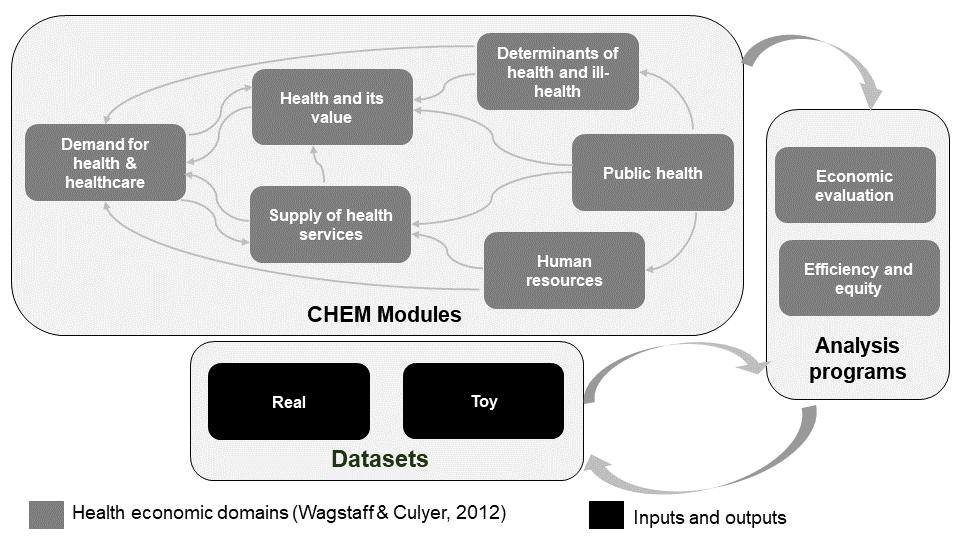
\includegraphics[width=400px,]{../Data/images/Figure1} \caption{High level summary of planned implementation of youth mental health economic model}\label{fig:fig1}

    \endfigure
\egroup 
\newpage

\newpage
\appendix
\counterwithin{figure}{section}
\counterwithin{table}{section}

\bibliography{bibliography.bib}


\end{document}
